\svnInfo $Id$

\section{Bus Design}
\label{sec:protocol}
During normal operation, \bus remains in Bus~Idle~(\ref{sec:protocol-idle}).
A transmission begins with Arbitration~(\ref{sec:protocol-arbitration}), then
Message Transmission~(\ref{sec:protocol-transmission}), then
Message~End~Sequence~(\ref{sec:protocol-end}),
and Message~Acknowledgement~(\ref{sec:protocol-ack}). A unique feature of \bus
is that both the Message~End~Sequence and the Message~Acknowledgement are
interpreted as start Bus~Reset~(\ref{sec:protocol-reset}) signals by any
forwarding nodes. All events except initiating arbitration occur on the rising
edge of {\tt CLK}.

The Bus~Reset signal may occur at any time and supersedes any current state,
resetting all nodes on a \bus. After receiving a Bus~Reset, \bus returns to
idle state.

\begin{figure*}[h!]
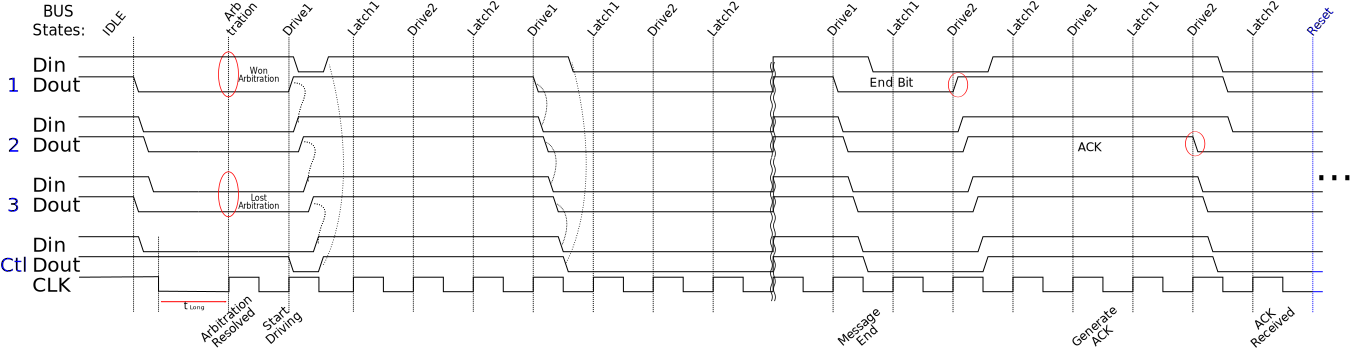
\includegraphics[width=\linewidth]{img/timing}
\caption{A complete transmission. In this system, there are
three member nodes (1, 2, and 3) and a control node. The data loop is connected
Ctl $\rightarrow 1 \rightarrow 2 \rightarrow 3 \rightarrow$ Ctl. This
demonstrates arbitration between member nodes 1 and 3, which node 1 wins. Node
1 then transmits data to node 2, which ACK's the data.}
\label{fig:transmission}
\end{figure*}

\subsection{Bus~Idle}
\label{sec:protocol-idle}
In \bus Bus~Idle, all lines ({\tt CLK}, {\tt DIN}, {\tt DOUT}) are high.
All member nodes are in forwarding state and the control node is waiting to
begin arbitration.

\subsection{Arbitration}
\label{sec:protocol-arbitration}
To begin arbitration, the bus must be in idle state.

To request to transmit on the bus, a node should pull its {\tt DOUT} line low.
All member nodes remain in forwarding state during arbitration, thus when
their {\tt DIN} line goes low, they are obligated to pull their {\tt DOUT}
line low. The control node, however, does {\bf NOT} pull its {\tt DOUT} line
low in response to its {\tt DIN} line going low. The control node only pulls
its {\tt DOUT} line low when it wishes to transmit on the bus. When the
control node's {\tt DIN} line goes low, it will pull the {\tt CLK} line low
and hold it low for some period $t_{long}$.

By the end of the period $t_{long}$, the effect of the arbitration is
achieved. A member node is in one of three possible states:
\begin{enumerate}
  \item {\tt CLK} low, {\tt DIN} high, {\tt DOUT} high -- Lost arbitration
    (didn't participate)
  \item {\tt CLK} low, {\tt DIN} high, {\tt DOUT} low -- Won arbitration
  \item {\tt CLK} low, {\tt DIN} low, {\tt DOUT} low -- Lost arbitration
    (either lost, or didn't participate)
\end{enumerate}
If the control node wishes to transmit on the bus, all member nodes will be in
the third state. Note this arbitration protocol introduces a {\em
topology-dependent priority}. Firstly, the control node has a greater priority
than any member node as its {\tt DOUT} will propagate around the entire data
loop. The priority of the member nodes is inversely related to their proximity
to the control node in the data loop. That is, the furthest node from the
control node, the node whose {\tt DIN} is connected to the control node's
{\tt DOUT}, has the highest priority of member nodes. The closest node to the
control node, the node whose {\tt DOUT} is connected to the control node's
{\tt DIN}, has the lowest priority.

At the end of $t_{long}$, the control node drives the {\tt CLK} line high. The
arbitration phase ends on this rising edge. Whichever node won the arbitration
transitions from a forwarding node to a transmitting node. If it is not the
transmitting or receiving node, the control node enters forwarding mode for
the duration of the transmission.

The rising edge that established the arbitration winner
is defined as a {\sc latch2} edge. This means the next clock edge will be a
{\sc drive1}, when the transmitting node should send the first bit of the
destination address.

\subsection{Message Transmission}
\label{sec:protocol-transmission}
During transmission, \bus alternates between the {\sc drive1}, {\sc latch1},
{\sc drive2} and {\sc latch2} states on every rising {\tt CLK} edge. 
Note, for forwarding (and receiving) nodes, the {\tt DIN} and {\tt DOUT} lines 
are {\bf NOT} clocked, nodes should forward data signals immediately.

The first rising edge after arbitration starts the first {\sc drive1} state.
After {\tt CLK} goes high, the transmitting node should set its {\tt DOUT}
line to {\tt 0} or {\tt 1} as appropriate. At the next rising edge, \bus
switches to {\sc latch1} state and nodes latch the value on their {\tt DIN}
lines. The next rising edge starts the {\sc drive2} state. The transmitting
node should \textsc{\textbf{FORWARD}}, not drive. During a normal
transmission, the value forwarded will not change, but if any node desires to
reset the bus, they may do so by setting the opposite bit during {\sc drive2},
initiating a Bus~Reset event\footnote{
  Caution must be taken by a resetting node to not introduce a false
  Message~End~Sequence. See the note in~\ref{sec:protocol-reset} for details.}
The final state is {\sc latch2} at the next rising edge, where the same bit is
read again, matching the bit read during {\sc latch1}.  It is at this
point---when the same bit has been received during {\sc latch1} and {\sc
latch2}---that the receiving layer records the incoming bit. The next clock
edge starts the sequence over, returning to {\sc drive1}.

The first sequence of bits pushed onto \bus are the {\em address} bits. All
nodes on a \bus should listen until their address:
\begin{itemize}
  \item Matches: Node promotes itself from forwarder to receiver.
  \item Does Not Match: Node remains forwarder for the rest of the
    transmission.
\end{itemize}

There is no protocol-level delineation between address and data bits. The
transmitting node sends address$+$data as a continuous stream of bits until
it terminates the message with a Message~End~Sequence.

\subsection{Message End Sequence}
\label{sec:protocol-end}
Picking up transmission from the last bit of data the transmitting node wishes
to send, the transmitting node pushes its last bit on its {\tt DOUT} line
during the {\sc drive1} state, and it is latched by \bus during the {\sc
latch1} and {\sc latch2} states.  At the next {\sc drive1} state, the 
transmitting node drives its {\tt DOUT} line low. This low bit is a sentinel 
stop bit---it is not part of the transmitted message, rather the beginning of 
the Message~End~Sequence. At the rising edge of the {\tt CLK} that starts the
{\sc latch1} state, all \bus nodes latch {\tt 0}. The next rising edge of the
{\tt CLK}, which starts {\sc drive2} state, the transmitting node drives its 
{\tt DOUT} line high. At the next rising {\tt CLK} edge, which starts the next 
{\sc latch2} state, nodes will observe that the data line differs from 
{\sc latch1} state. All forwarding nodes will treat this transition as a 
Bus~Reset signal. The receiving and control nodes, however, will recognize 
this sequence as a Stop.

At the next rising edge after transmitting the Stop sequence, the transmitting
node should begin forwarding its {\tt DIN} to its {\tt DOUT}.

After any Bus~Reset (which Stop qualifies as), the control node will drive 2
more pulses on the {\tt CLK} line. For forwarding nodes not participating in
this transaction, these are the pulses required to transition them from {\sc
reset} to {\sc idle}. For the transmitting and receiving nodes, the {\sc
drive} / {\sc latch} alternation continues.

\subsection{Message Acknowledgement}
\label{sec:protocol-ack}
After the Stop message, the receiving layer is responsible for sending a
message acknowledgement. The message was determined to be a Stop at the {\sc
Latch2} that ended the previous cycle.

At the next rising clock edge, a {\sc drive1}, the {\em receiving} layer
should drive a {\tt 1} (Note that this will not create an edge yet as the bus
should already be high from the end of the Stop sequence). The value {\tt 1}
is latched by \bus at the next clock edge during {\sc latch1}. At the next
clock edge, {\sc drive2}, the receiving layer should drive {\tt 0} if it
wishes to acknowledge the transmission. The acknowledgement is confirmed at
the next clock edge, {\sc latch2}.

This is a relatively fast turnaround for the receiving node. It has from {\sc
latch2} when it detects the Stop condition until the next {\sc drive2} to
determine whther or not it wishes to acknowledge the transmission. Designers
should take care to ensure the acknowledge signal logic can be generated in
half a bit time (2 clock pluses).

It is important that the receiving node continues to monitor its {\tt DIN}
line during the Message~Acknowledgement sequence. In particular, during the
{\sc Latch1} phase of the acknowledgement sequence, if the {\tt DIN} value is
{\tt 0} instead of {\tt 1}, the receiving node {\em cannot} acknowledge the
message, and the entire transaction should be aborted, and receiving node
should return to the Forwarding.{\sc reset} state. This condition may occur
when an asychronous Bus~Reset event is triggered.

After Acknowledgement/Bus~Reset sequence, the control node will drive one
full cycle (4 pulses on the {\tt CLK} line), after which the \bus returns to
Bus~Idle.

\subsection{Bus Reset}
\label{sec:protocol-reset}
The \bus cycles through {\sc drive1}, {\sc latch1}, {\sc drive2}, and {\sc
latch2} on every rising clock edge.  Coming from Bus~Idle, the first rising
clock edge is defined as a {\sc latch2 state}.
The transmitting node sets {\tt DOUT} to
its new value on the next rising edge, the {\sc drive1} state.

If {\tt DIN} has changed between the {\sc Latch1} state and the {\sc latch2}
state, this indicates a start of Bus~Reset sequence. Upon receipt of start of
Bus~Reset, all member nodes should switch to the Forwarding.{\sc reset} state,
{\bf except}
\begin{itemize}
  \item A transmitting node sending a Message~End~Sequence.
  \item A receiving node receiving a Message~End~Sequence.
\end{itemize}
Both transmitter and receiver should revert to forwarding.{\sc reset}
after sending / receiving a Message~Acknowledgement. After the
Message~End~Sequence and Message~Acknowledgement are complete, all member
nodes should be in Forwarding.{\sc reset}, waiting for four more clock pulses
to transition to Forwarding.{\sc idle}.

When a Bus~Reset is received, the control node will drive four more clock
pulses---one more complete cycle.
Depending on the {\tt DIN} during these cycles, the control node will:
\begin{table}[h!]
  \def\arraystretch{2}
  \begin{tabularx}{\linewidth}{| c | X |}
    \hline
    1 1 & Return to Bus~Idle. \\ \hline
    0 1 & This corresponds to the Stop sequence. The sequence should only
    occur once be transaction, if more are detected, the control node will
    begin forcefully resetting the bus, as outlined below.\\ \hline
    1 0 & This corresponds to the Acknowledgement sequence. This sequence
    terminates a transaction. After an Acknowledgement, the control nodes sets
    its {\tt DOUT} line high, and issues four more clock pulses, returning all
    nodes to Bus~Idle. \\ \hline
    0 0 & This state should not occur in normal operation. In response, the
    control node will drive four more pulses, ignoring its {\tt DIN} line and
    generating a Bus~Reset signal. It will then generate four more clock
    pulses with its {\tt DOUT} line high, repeating this process until it
    samples four 1's on its {\tt DIN} line. \\ \hline
  \end{tabularx}
\end{table}

\noindent
\textbf{\em IMPORTANT:} If a node initiates Bus~Rest during the transmission
of a {\tt 0} bit and is not the receiving node, it will have introduced a
false Message~End~Sequence. The node issuing the reset is responsible for
driving a {\tt 0} during the next {\sc Drive1} and {\sc Drive2} cycles,
ignoring its {\tt DIN}.  A receiving node attempting to ACK the message will
detect this and fail the transaction appropriately. This will cause the
control layer to detect an erroneous state and issue one more reset cycle,
driven by the control layer.

%\begin{quote}
%\begin{bytefield}{32} \\
%\colorbitbox{lightgreen}{8}{Message Type} &
%\colorbitbox{lightred}{8}{Event ID} &
%\colorbitbox{lightcyan}{8}{Length} &
%\bitbox{8}{[Message Data...]} &
%\end{bytefield}
%\end{quote}


